\subsection*{Axolotli} % (fold)
\label{sub:axolotli}

\begin{multicols}{2}

Na samotce byla nuda. Bylo tam tolik komárů a vos jako Somálců v budce když tam hodíš piškot. Na DVD jsme udělali fakt hodně pudinku a nikdo ho nechtěl  stejně jako na manévrech, kde jsme udělali fakt hodně pudinku ve kterym byly úplně nechutný sušený, ale znovu rehydrovaný banány. Vyhráli jsme bodování a jako odměnu jsme dostali utopence...
P.S. Linux je lepší než Windows

\podpis{Einstein}




Tři orlí pera- samotka:\\
Rád vzpomínám na tábor. Na tomto táboře jsmem se jeden den nejvíc nudil a to bylo poslední zkouška třích orlích per, byla to zkouška samotky. Byla to hrozná nuda, spal jsem asi do desíti hodin přes noc mi kus chleba sežrala myš kterou jsem pak večer viděl. Tři orlí pera jsem udělal.

\podpis{Bobeš}

\columnbreak

Rád vzpomínám na tábor. Na tomto táboře bylo nejzajímavější, když jsme měli družinkáč. Bylo to zajímavé, protože Einstein a H-hruška drželi hladovku a já jsem mlčel. Tak jsme čekali až do půlnoci a pak jsme začali smažit řízky. Jídlo jsme jedli na mé a Einsteinově hlídce. Bylo to moc dobré. Jsem moc rád, že nám uďové dovolili na družinkáči řízky.

\podpis{Picasso}


Rád vzpomínám na tábor. Jedna z věcí na kterou rád vzpomínám je genderový program. Program měl na starosti Hafík a Kibitz. Ty nám připravili workout a jiné mužské záležitosti. Ze začátku jsme “posilovali”. Poté jsme šli sbírat proteiny. Jako proteiny jsme vzali kobylky. Následně jsme je usmažili. Podávali se buď na sladko nebo na slano. Na konec se pořádali řeckořímské zápasy.

\podpis{Hahruška}
\end{multicols}

\begin{center}

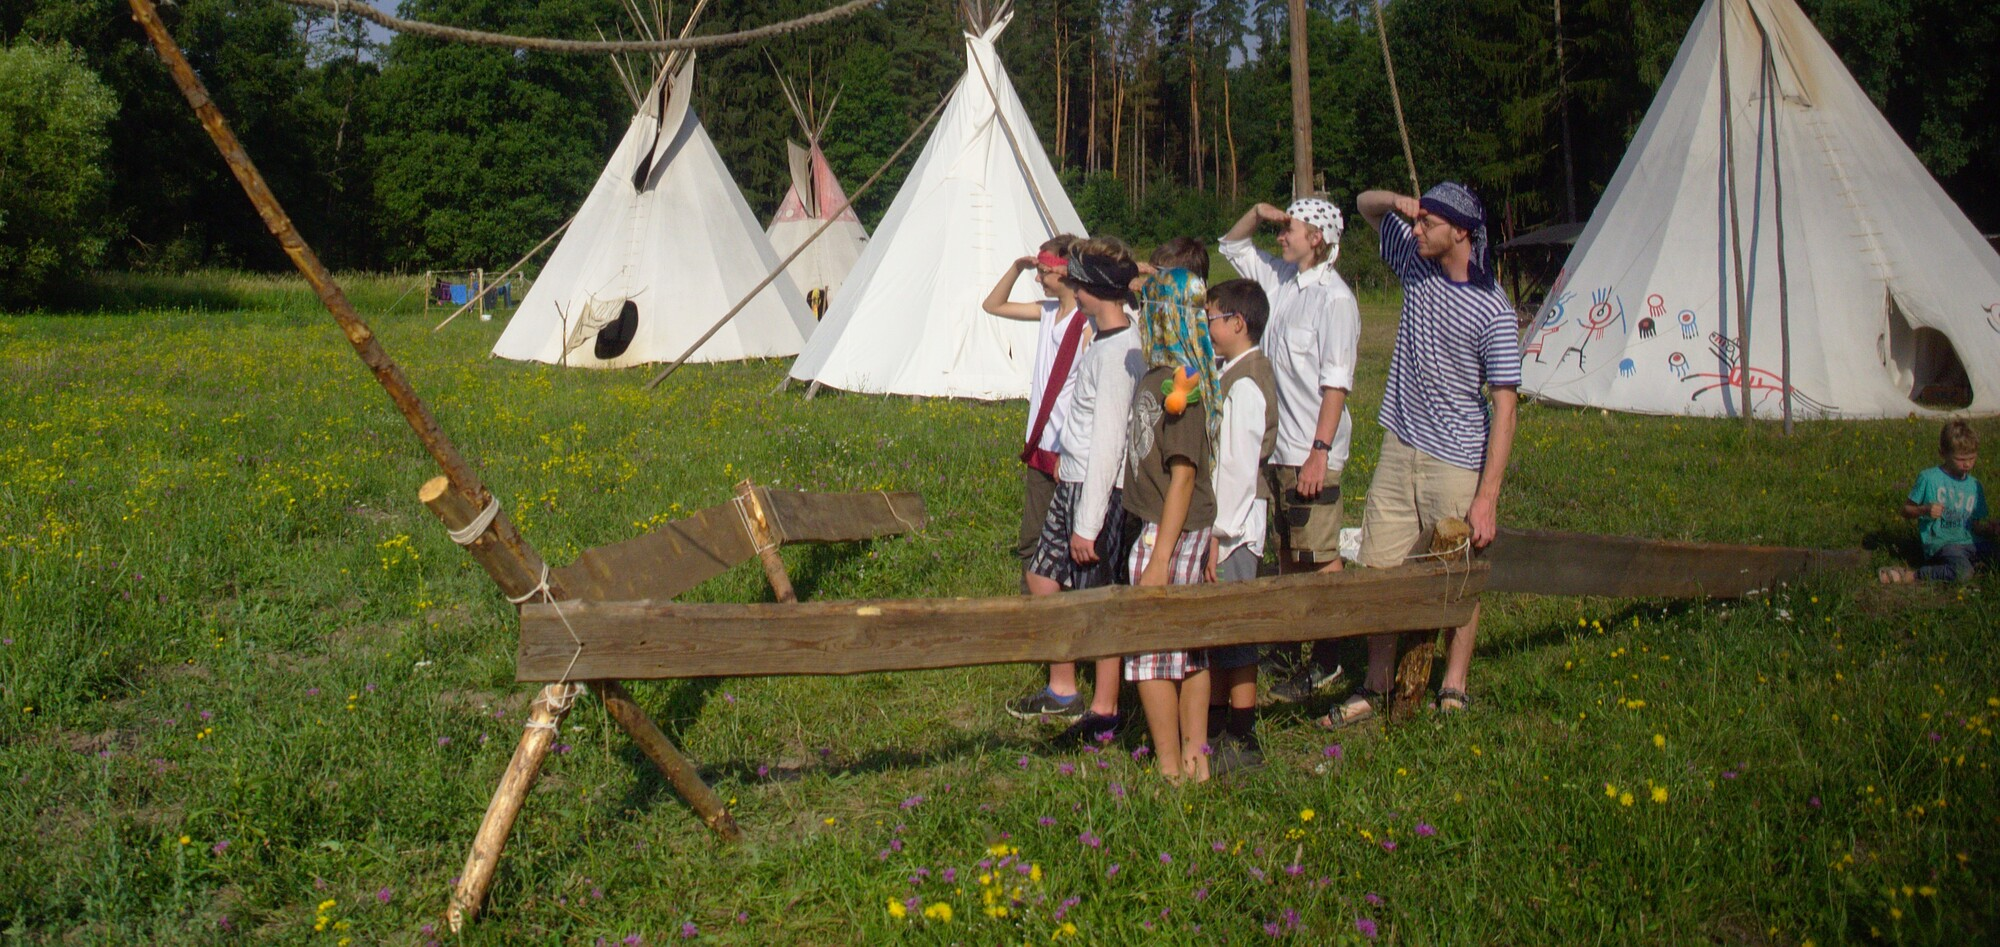
\includegraphics[width=10cm]{img/druziny/axolotli.jpg}

\end{center}

%\clearpage

% subsection axolotli (end)
